
This thesis is motivated by the results presented in \parencite{michelot_langevin_2019}. In the article, a model for animal movement based on the Langevin process is presented, and it is shown how this model can be used to estimate the UD of an animal. A problem that arises when the time between observations is large and, which is discussed by \parencite{michelot_langevin_2019}, is that as the time between observations increases, there is an increasing bias in the parameter estimates. In this section, the model used by \parencite{michelot_langevin_2019} is presented and some of the results of the article are reproduced.



\section{The Langevin Process}
The Langevin process is a form of diffusion process described in Section~\ref{sec: diffusion processes}, and takes the form

\begin{equation}
    d\textbf{X}_t = \frac{1}{2} \nabla \log(\pi(\textbf{X}_t))dt + d\textbf{B}_t, \ \textbf{X}_0 = \textbf{x}_0.
    \label{eq:Langevin equation}
\end{equation}


$\pi$ is referred to as the UD, and the drift term $\nabla log(\pi(\textbf{X}_t))$ steers the particle $X_t$ to areas of $\pi$ with a grater value. In an animal setting, this can be interpreted as the tendency of an animal to be attracted to certain areas over others.



\parencite{dalalyan_theoretical_2017} states that under the conditions that $\pi$ is convex and has a Lipschitz continuous gradient, the diffusion equation has a unique solution, which is a continuous-time Markov process with $\pi$ as the stationary distribution of $X_t$. This means that the time an animal spends in an area over the long term is determined by the UD, and we can write that

\begin{equation}
    P(\textbf{X}_t \in A ) = \int_A \pi(\textbf{z})d\textbf{z}.
\end{equation}


To make use of the Langevin movement model in practice, there needs to be a parameter to control the speed of the process. This is because, although two animals might have the same UD, the speed at which they travel may be different. In the Langevin process \eqref{eq:Langevin equation} the speed of a particle is determined by the UD, so two particles with the same distribution. In reality, two animals can have the same UD, but still have different speeds. \parencite{roberts_optimal_1998} adds a speed parameter $\gamma^2$ to the Langevin process, which can change the speed of diffusion. The resulting process can be expressed by the equation

\begin{equation}
    d\textbf{X}_t = \frac{\gamma^2}{2} \nabla \log(\pi(\textbf{X}_t))dt + \gamma d\textbf{B}_t, \ \textbf{X}_0 = \textbf{x}_0.
    \label{eq:Langevin with speed}
\end{equation}


If the solution to the original Langevin process \eqref{eq:Langevin equation} is $\textbf{X}^*_t$ and the solution to the Langevin process \eqref{eq:Langevin with speed} with speed $\gamma^2$ is $\textbf{X}_t$, then their relationship can be expressed as $\textbf{X}_t = \textbf{X}^*_{\gamma^2 t}$. This means that the parameter scales the time of the process, making it faster or slower.


\section{Resource Selection Functions}

Covariates can be included in the model by specifying the UD. For this, we can use a Resource Selection function (RSF). An RSF is a function that expresses the probability of an animal utilizing a resource over all other resources in the area being studied. \textcite{michelot_langevin_2019} uses an RSF of the form


\begin{equation}
    \pi(x|\beta) = \frac{exp(\sum_{i=1}^n\beta_i c_i(x))}{\int_\Omega exp(\sum_{i=1}^n\beta_i c_i(z))dz}.
    \label{eq: resource selection function}
\end{equation}

$\Omega$ is the area of study, $C_i(x)$ are the spatial covariates. the covariates can represent geographical or environmental factors that are distributed in space and that we want to study. $\beta_i$ are the coefficients that scale the spatial covariates. By using the RSF as the UD of \eqref{eq:Langevin with speed}, we can find how the various covariates affect the animal movement, and which covariates are attractive. The slope term of \eqref{eq:Langevin with speed} then becomes

$$
    \nabla log(\pi(x|\beta)) = \nabla log(\frac{exp(\sum_{i=1}^n\beta_i c_i(x))}{\int_\Omega exp(\sum_{i=1}^n\beta_i c_i(z))dz}) =\sum_{i=1}^n \beta_i \nabla c_i(x).
$$



Environmental covariates are usually not expressed as analytical functions, as is assumed for the Langevin model and the Euler approximation of it. Most often, they are stored as point data on a grid. To find the value of the covariates at points outside the grid, we therefore have to interpolate from the grid. We can find values for the gradient of the covariates using the method described in Subsection~\ref{subsec: gradient estimation}


\section{Likelihood Approximation of Langevin Process}
\label{sec: Likelihood Approximation of the Langevin Process}
If we observe the positions of the animal at locations $\textbf{X}_i$ at times $t_i$ for $i=1,\dots , K$, we can express the likelihood of the parameters $\bm{\beta}$ and $\gamma^2$ given these jumps using a transition function $q_{\Delta_i}(\textbf{X}_{i+1} | \textbf{X}_i)$, where $\Delta_i = t_{i+1} - t_i$ is the change in time between states. Because of the Markov property of the solution to the Langevin diffusion equation, we can express the entire likelihood of the animal movement as

\begin{equation}
    L(\bm{\beta}, \gamma^2 | \textbf{X}) = \prod_{i=0}^{K-1} q_{\Delta_i}(\textbf{X}_{i+1} | \textbf{X}_i, \theta).
    \label{eq: Langevin likelihood}
\end{equation}

However, there is a problem with this approach. For the Langevin diffusion, there is no closed form expression for $q_\Delta$\parencite{gloaguen_stochastic_2018}. Instead of using the exact likelihood, pseudo-likelihood methods can be used instead. However, one of the most used methods for approximating SDE is the EM method described in \ref{subsec: Euler-Maruyama}. The Langevin process transition will then be approximated as

$$
    \textbf{X}_{i+1} = \textbf{X}_i + \frac{\gamma^2 \Delta_i}{2}\nabla log(\pi(\textbf{X}_i)) + \sqrt{\Delta_i}\gamma \bm{\epsilon}_i, \ \ i = 1,\dots , K-1,
$$

where $\bm{\epsilon}_i$ are standard two-dimensional Gaussian distributions. Using this approximation, we get the transition densities 

$$
q_{\Delta_i}(\textbf{x}_{i+1} | \textbf{x}_i, \theta) = \mathcal{N}(\textbf{x}_i + \frac{\gamma^2 \Delta_i}{2}\nabla \log(\pi(\textbf{x}_i)), \Delta \gamma^2 I_{2*2}),
$$

and we get the likelihood approximation

$$
L(\bm{\beta}, \gamma^2 | \textbf{X}) = \prod_{i=0}^{K-1} \mathcal{N}(\textbf{X}_i + \frac{\gamma^2 \Delta_i}{2}\nabla \log(\pi(\textbf{X}_i)), \Delta_i \gamma^2 I_{2*2}).
$$

\parencite{iacus_simulation_2008}.






\section{Estimating Parameters}
\label{sec: estimating parameters}
we can use the Langevin process transition approximation from Subsection~\ref{sec: Likelihood Approximation of the Langevin Process} to estimate the parameters used in the model. If we let $\textbf{Y}_i = (\textbf{X}_{i+1} - \textbf{X}_i)/\sqrt{\Delta_i}$ be the increments of the observed Langevin process, we get $\textbf{Y}_i = \frac{\gamma^2}{2}\nabla log(\pi(\textbf{X}_i)) + \gamma \bm \epsilon_i$. In the case where we are using a RSF with covariates $j$, we can write $\nabla log(\pi(\textbf{X}_i)) = \sum_{k = 1}^j \beta_k \nabla c_k(\textbf{X}_i)$, so we get

$$
    \textbf{Y}_i = \frac{\gamma^2 \sqrt{\Delta_i}}{2}\sum_{k = 1}^j \beta_k \nabla c_k(\textbf{X}_i) + \gamma \bm \epsilon_i.
$$

Let $\textbf{Y}_i = (Y_{i,1}, Y_{i,2})$ be the two-dimensional process with $\bm \epsilon_i =(\epsilon_{i,1}, \epsilon_{i,2})$, and let

$$
    \mathbf{Y} = \begin{pmatrix}
        Y_{0,1} \\
        \vdots \\
        Y_{K-1,1}\\
        Y_{0,2}\\
        \vdots\\
        Y_{K-1,2}
    \end{pmatrix} , \    
    \mathbf{D} = \frac{1}{2} 
    \begin{pmatrix}
        \frac{\partial c_1(x_0)}{\partial z_1} & \dots & \frac{\partial c_j(x_K)}{\partial z_1} \\
        \vdots & & \vdots \\
        \frac{\partial c_1(x_K)}{\partial z_1} & \dots & \frac{\partial c_j(x_K)}{\partial z_1} \\
        \frac{\partial c_1(x_0)}{\partial z_2} & \dots & \frac{\partial c_j(x_K)}{\partial z_2} \\
        \vdots & & \vdots \\
        \frac{\partial c_1(x_K)}{\partial z_2} & \dots & \frac{\partial c_j(x_K)}{\partial z_2}
    \end{pmatrix} , \
    \mathbf{E} =\begin{pmatrix}
        \epsilon_{0,1} \\
        \vdots \\
        \epsilon_{K-1,1}\\
        \epsilon_{0,2}\\
        \vdots\\
        \epsilon_{K-1,2}
    \end{pmatrix}.
$$


We can then write $\mathbf{Y} = \mathbf{Z} \bm{\nu} + \mathbf{E}$, where $\mathbf{Z} = \mathbf{T}_\Delta D$ and $\mathbf{T}_\Delta$ is the $2K\times 2K$ matrix with diagonal elements $\sqrt{\Delta_i}$ for $i=1, \dots, K$ and $\sqrt{\Delta_{i-K}}$ for $i=K+1,\dots 2K$. Now, the problem of finding estimates for $\bm{\nu} = \gamma^2 \bm{\beta}$ is that of solving a linear regression problem, so we get

$$
\bm{\hat{\nu}} = (\mathbf{Z}^T\mathbf{Z})^{-1}\mathbf{Z}^T \mathbf{Y}.
$$

Estimates for the speed parameter $\gamma^2$ and $\bm{\beta}$ can be found by using
$$
\hat{\gamma}^2 = \frac{1}{2K-j} \lVert \mathbf{Y} - \mathbf{\hat{Y}} \rVert^2_2, \ 
\bm{\hat{\beta}} = \frac{\bm{\hat{\nu}}}{\hat{\gamma}^2}.
\label{eq: michelot estimates}
$$



\section{Assessment of the Model}

\subsection{Simulating Covariates}
To study the Langevin movement model, \parencite{michelot_langevin_2019} simulates the Langevin process using two covariates on a grid simulated from  Matérn Gaussian random fields, and one covariate which is the square of the euclidean distance to the origin. The last of these covariates ensures that the Langevin process tracks do not exit the study area. Simulating covariates from a Matérn field is memory and time intensive. Because of this, I instead use Perlin noise simulated using the R package "ambient" with frequency parameter 0.05 and scaled by 3. The two covariates simulated using Perlin noise are shown in figure~\ref{fig:covariate plots}. In addition, the figure displays the UD found using the formula for a RSF \eqref{eq: resource selection function} with all three covariates.

\begin{figure}[H]% 
    \centering
    \subfloat[\centering Perlin noise covariate simulation\label{fig: cov2}]{{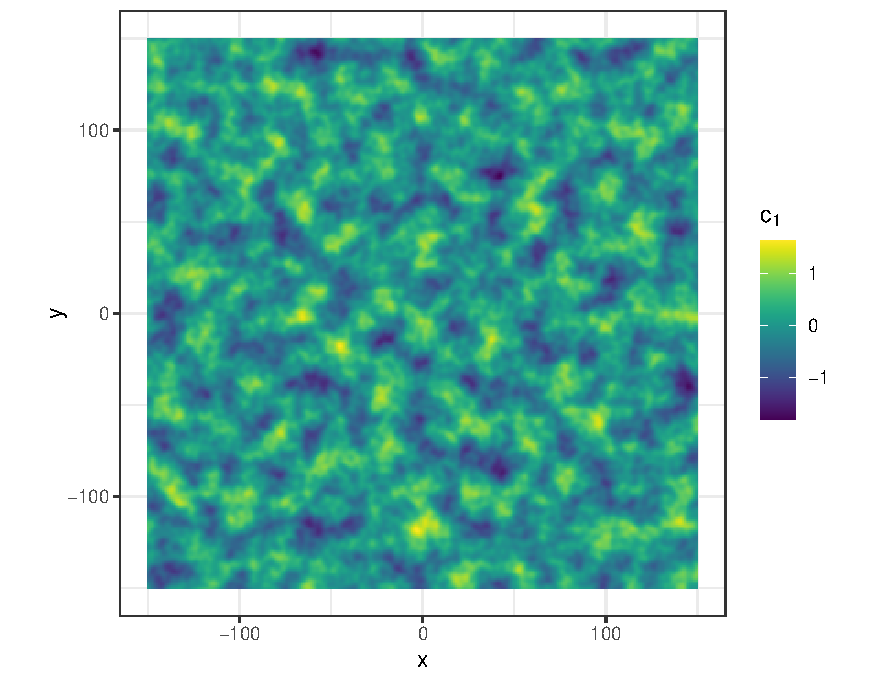
\includegraphics[width=.45\linewidth]{Images/background/covariate 1 plot.pdf} }}%
    \qquad
    \subfloat[\centering Perlin noise covariate simulation\label{fig: cov2}]{{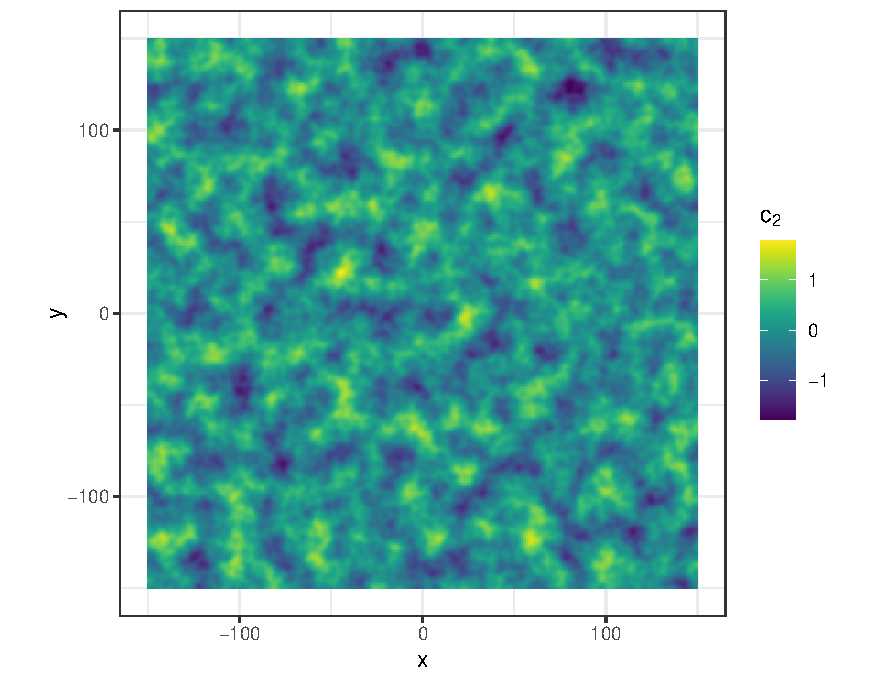
\includegraphics[width=.45\linewidth]{Images/background/covariate 2 plot.pdf} }}%
    \qquad
    \subfloat[\centering UD\label{fig: UD}]{{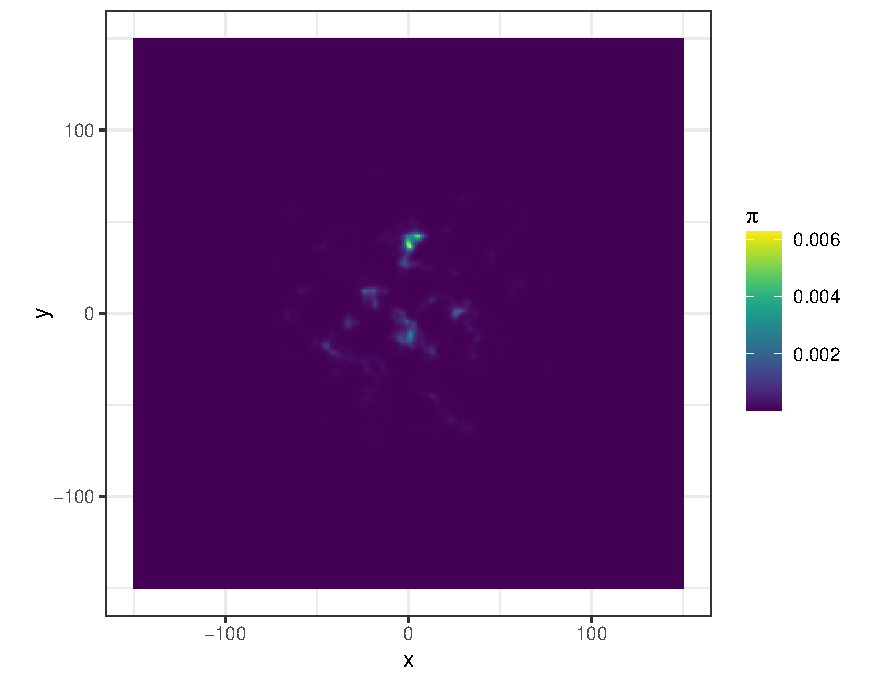
\includegraphics[width=.45\linewidth]{Images/background/UD plot.pdf} }}%    
    \caption[covariate and UD plots]{(a), (b): figures showing covariates simulated using Perlin noise with frequency parameter 0.05. (c): RSF using covariates (a), (b) and square of Euclidean distance to origin.}%
    \label{fig:covariate plots}%
\end{figure}


The code for generating Figure \ref{fig:covariate plots} can be found in the git hub repository in the file "covariate plot.R". The figure shows that the covariates generated by the Perlin noise contains multiple peaks and valleys, which means that it can be used to simulate complex movements for the Langevin process. Figure \ref{fig: UD} shows the combined UD. The third covariate ensures that the simulated tracks do not drift too far from the center of the map, where the slope of the UD is not defined. It also simulates how one might think that an animal might stay around its home range. 


\subsection{Accuracy of the Approximation}
To demonstrate the accuracy of the Euler approximation at various step intervals, \parencite{michelot_langevin_2019} uses the Metropolis adjusted Langevin algorithm (MALA) \parencite{roberts_exponential_1996}. This algorithm uses the EM method as a proposal in the metropolis-Hastings algorithm and then uses the UD as the target distribution. This ensures that the stationary distribution of the EM method is actually the UD. The EM method only approximates the Langevin process when the time intervals are small, so we should expect the acceptance rate of MALA to be small when the time intervals are large and close to one when the time intervals are small. Because of this, we can use the MALA acceptance rate to judge at which time resolution the EM method becomes a good approximation of the Langevin process. \parencite{michelot_langevin_2019} simulates Langevin tracks at 9 resolutions $\Delta_t\in \{ 0.01, \ 0.02, \ 0.05, \ 0.1, \ 0.2, \ 0.5, \ 1, \ 2, \ 5 \}$ using the speed parameter $\gamma^2 = 5$, the covariates from Figure\ref{fig:covariate plots} and simulating up to time $T=1000$. They then computed the average acceptance rate for each of the resolutions. The resulting acceptance rates are shown in Figure~\ref{fig:MALA}, and is reproduced using the code from \parencite{michelot_langevin_2019}. The code can be found in the github repository in Appendix~\ref{Appendix: github repo} under the file name "MALA figure.R"

\begin{figure}[H]
    \centering
    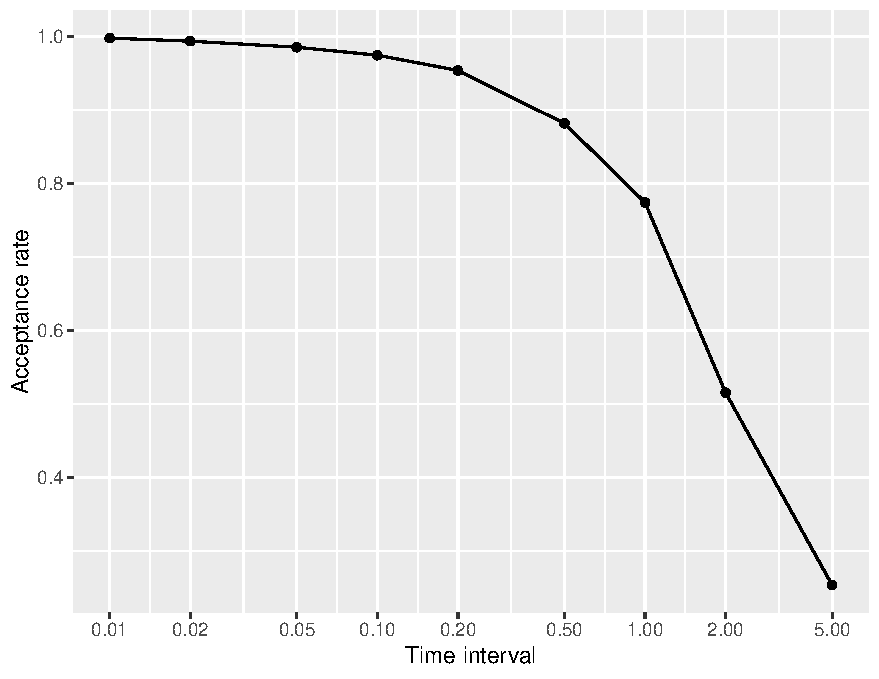
\includegraphics[width=\linewidth]{Images/background/MALArates.pdf}
    \caption[MALA acceptance rates]{Acceptance rate for the metropolis adjusted Langevin algorithm for various values of increments of the EM approximation. The X-axis is on log-scale.}
    \label{fig:MALA}
\end{figure}


Figure~\ref{fig:MALA} shows that for a time interval of $\Delta_t =0.01$, the acceptance rate of MALA is close to 1. This would indicate that at this resolution the EM method is a good approximation of the Langevin process. However, as the time interval increases in size, the EM method becomes a worse approximation of the Langevin process.


\subsection{Underestimation of Parameters}

With the UD in Figure~\ref{fig: UD}, we can use the EM method to simulate tracks from the Langevin model and see how the estimated values of the parameters used compare to their actual values for different time increments between observations. To do this, 100 Langevin tracks were simulated using a resolution of $0.01$ with the Perlin covariates in Figure~\ref{fig:covariate plots} and the speed parameter $\gamma^2 = 5$. The tracks were then thinned to give resolutions $\Delta_t \in \{0.01, \ 0.02, \ 0.05, \ 0.1, \ 0.2, \ 0.5, \ 1 \}$ between the observations and then shortened so that they contained 5000 observations each, giving 100 tracks for each of the resolutions. The parameters $\gamma^2$ and $\bm \beta$ were then estimated using \eqref{eq: michelot estimates}. The resulting estimates are displayed as box plots in Figure~\ref{fig:EM_thin_boxplot}.


\begin{figure}[H]
    \centering
    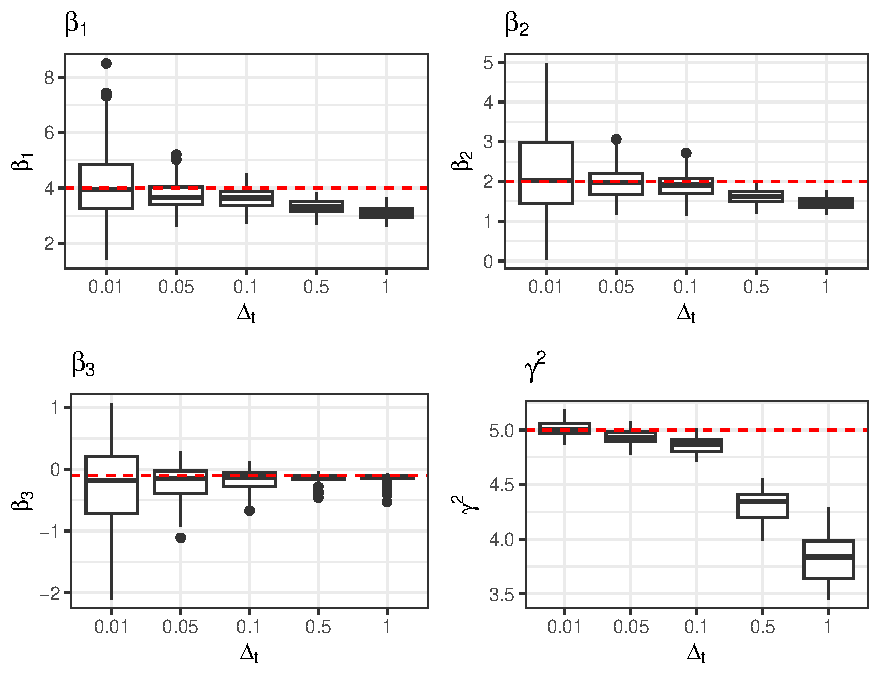
\includegraphics[width=\linewidth]{Images/background/varying dt EM boxplot.pdf}
    \caption[Euler-Mauryama estimates]{Box plots of estimated parameters using the EM method on 100 Langevin tracks simulated at a resolution of $0.01$, then thinned to $\Delta_t \in \{0.01, \ 0.05, \ 0.1, \ 0.5, \ 1\}$ and shortened to 5000 observations. The number of steps used in the predict step was $\Delta_t/0.01-1$. Red line indicates the true value of the parameters.}
    \label{fig:EM_thin_boxplot}
\end{figure}


The code for generating Figure~\ref{fig:EM_thin_boxplot} can be found in the GitHub repository under the name "varying dt EM estimates.R". Figure~\ref{fig:EM_thin_boxplot} shows that there is an increasing bias in the estimates of $\bm \beta$ as the time increments between the observations increases. Figure~\ref{fig:MALA} shows that for larger time increments, the EM method is no longer a good approximation for the Langevin process likelihood. This explains why the estimates are not unbiased. \parencite{michelot_langevin_2019} explains the bias by the fact that when $\Delta_t$ is large, a lot of the movement in accordance with the UD is lost, making it appear flatter than it actually is. A track might follow the slope of the UD well, but when the intermediate states are removed, that information disappears. This flattening could be an explanation for why the approximation gives estimates that are closer to zero than the true values of the parameters. 


Another observation is that the variance of the estimates decreases as the size of the time increments increases. \parencite{michelot_langevin_2019} explains this by the fact that, for larger increments, the observations are more spaced out, meaning that they explore more of the map. When more of the covariate range is explored, the variance of the coefficient estimates is reduced. The same bias is also observed in the $\gamma^2$ estimates. The underestimation here might be because the distance traveled seems smaller when we have coarser resolutions, since some of the movement is removed. Unlike what is observed for $\bm \beta$, the variance of the estimates of $\gamma^2$ increase as the time increments increase.

